\section{Calcolo vettoriale e tensoriale in coordinate curvilinee}

Dopo aver introdotto alcuni concetti di algebra tensoriale nella sezione precedente, viene fatta una breve introduzione al calcolo tensoriale. In questa sezione vengono introdotte alcune definizioni e operatori differenziali necessari per descrivere campi (funzioni dipendenti dallo spazio) tensoriali. Si ricavano le espressioni in coordinate degli operatori rispetto a sistemi di coordinate curvilinee generali. Si introducono poi i sistemi di coordinate curvilinee ortogonali. Infine, si scrivono le espressioni di alcuni operatori differenziali e, come utile esempio per un corso di fluidodinamica, le equazioni di Navier-Stokes in un sistema di coordinate cilindriche.
Per aiutare la comprensione dell'argomento, i concetti generali verranno specializzati ad alcuni sistemi coordinate particolari, come le coordinate cartesiane o cilindriche.

Lavoriamo per semplicità in uno spazio tridimensionale, descritto completamente
 dalle tre coordinate $\left\{q^1, q^2, q^3\right\}$: il vettore posizione $\bm{x}$ sarà quindi una funzione
 delle tre coordinate $q^i$:
 \begin{equation}
  \bm{x} = \bm{x}(q^1, q^2, q^3)
 \end{equation}
 Si suppone che la trasformazione di coordinate da $\bm{x}$ a $\left\{q^1, q^2, q^3\right\}$ sia biunivoca. Vengono fornite ora le definizioni di curve coordinate, superfici coordinate e base naturale indotta dalla parametrizzazione dello spazio.

\begin{definition}[Curve coordinate]
 Le curve coordinate passanti per il punto $\bm{x}_0=\bm{x}(q_0^1, q_0^2, q_0^3)$ sono le curve ottenute al variare di una coordinata, tenendo fisse le altre due
 \begin{equation}
 \begin{cases}
  \ell_1 : \quad \bm{x} = \bm{x}(q^1, q_0^2, q_0^3) \\
  \ell_2 : \quad \bm{x} = \bm{x}(q_0^1, q^2, q_0^3) \\
  \ell_3 : \quad \bm{x} = \bm{x}(q_0^1, q_0^2, q^3) .
 \end{cases}
 \end{equation}
\end{definition}
 
\begin{definition}[Superfici coordinate]
 Le superfici coordinate passanti per il punto $\bm{x}_0=\bm{x}(q_0^1,q_0^2,q_0^3)$ sono le superficie descritte da due coordinate, tenendo fissa l'altra
 \begin{equation}
 \begin{cases}
  S_1 : \quad \bm{x} = \bm{x}(q_0^1, q^2, q^3) \\
  S_2 : \quad \bm{x} = \bm{x}(q^1, q_0^2, q^3) \\
  S_3 : \quad \bm{x} = \bm{x}(q^1, q^2, q_0^3) .
 \end{cases}
 \end{equation}
\end{definition}
 
\begin{definition}[Base naturale]
 Per ogni punto dello spazio tridimensionale $\bm{x}=\bm{x}(q^1,q^2,q^3)$, viene definita la base naturale $\{ \bm{b}_i \}_{i=1:3}$, i cui elementi sono le derivate parziali del vettore posizione rispetto alle coordinate $q^i$,
 \begin{equation}
  \bm{b}_i = \dfrac{\partial \bm{x}}{\partial q^i} . %\quad,\qquad \bm{b}^i = g^{ik} \bm{b}_k
 \end{equation}
\end{definition}
  La base reciproca $\{ \bm{b}^i \}_{i=1:3}$ della base naturale viene definita tramite la definizione (\ref{eqn:defBaseReciproca}), cioé $\bm{b}^i \cdot \bm{b}_j = \delta_j^i$.

\begin{example}[Coordinate cartesiane]
 La posizione di un punto nello spazio tridimensionale viene definito dalle tre componenti $(q^1, q^2, q^3)=(x,y,z)$ nel sistema di coordinate cartesiane. Le curve coordinate sono rette parallele agli assi, mentre le superfici coordinate sono dei piani perpendicolari agli assi. I vettori della base naturale sono i tre versori $\bm{\hat{b}}_x = {\hat{x}}$, $\bm{b}_y = \bm{\hat{y}}$, $\bm{b}_z = \bm{\hat{z}}$ allineati con le linee coordinate, costanti in tutto lo spazio.
\end{example}

\begin{example}[Coordinate cilindriche]
 La posizione di un punto nello spazio tridimensionale viene definito dalle tre componenti $(q^1, q^2, q^3)=(r,\theta,z)$ nel sistema di coordinate cilindriche, come raffigurato in figura \ref{fig:cylCoord}. Le curve coordinate $\bm{x}(r_0,\theta_0,z)$ sono delle linee parallele all'asse $z$, le curve coordinate $\bm{x}(r_0,\theta,z_0)$ sono delle circonferenze con centro sull'asse $z$, mentre le curve coordinate $\bm{x}(r,\theta_0,z_0)$ sono dei raggi (semirette) perpendicolari all'asse $z$. Le superfici coordinate $S_3=S_z$ sono dei piani perpendicolari all'asse $z$, le superfici coordinate $S_2=S_{\theta}$ sono dei semipiani delimitati dall'asse $z$, le superfici coordinate $S_1 = S_r$ sono dei cilindri con asse coincidente con l'asse $z$, come raffigurato in figura \ref{fig:cylCoord}\subref{fig:cylCoord:a}. I vettori della base naturale non sono costanti in spazio. \'E possibile calcolarli, esprimendo il vettore posizione in coordinate cartesiane e in coordinate cilindriche. In particolare $\bm{x} = x \bm{b}_x + y \bm{b}_y + z \bm{b}_z$, con
\begin{equation}
 \begin{cases}
  x = r \cos \theta \\   y = r \sin \theta \\ z = z .
 \end{cases}
\end{equation}
I vettori della base naturale possono essere calcolati inserendo queste espressioni nella formula che descrive la posizione nella base cartesiana, costante in spazio e quindi con derivate spaziali nulle. In figura \ref{fig:cylCoord}\subref{fig:cylCoord:b} sono rappresentati i vettori della base naturale
\begin{equation}
 \begin{cases}
  \bm{b}_1 = \bm{b}_r = \dfrac{\partial \bm{x}}{\partial r} = \cos \theta \bm{b}_x + \sin \theta \bm{b}_y  = \bm{\hat{r}} \\
  \bm{b}_2 = \bm{b}_{\theta} = \dfrac{\partial \bm{x}}{\partial \theta} = -r \sin \theta \bm{b}_x + r \cos \theta \bm{b}_y = r \bm{\hat{\theta}}\\
  \bm{b}_3 =  \bm{b}_z = \bm{\hat{z}} ,
 \end{cases}
\end{equation}
avendo introdotto i versori $\bm{\hat{r}} = \cos \theta \bm{b}_x + \sin \theta \bm{b}_y$, $\bm{\hat{\theta}}= -\sin \theta \bm{b}_x + \cos \theta \bm{b}_y$, comunemente utilizzati per descrivere i problemi in geometria cilindrica.
\begin{remark}
 I vettori della base naturale indotta dalle coordinate cilindriche \textbf{non} è costante nello spazio, è ortogonale (come vedremo nella prossima sezione) ma \textbf{non} è ortonormale e non ha dimensioni fisiche omogenee: mentre i vettori $\bm{b}_r$ e $\bm{b}_z$ hanno modulo 1, il vettore $\bm{b}_\theta$ ha modulo $r$ ed ha le dimensioni fisiche di una lunghezza.
\end{remark}
\end{example}

\begin{figure}
\subfloat[][\emph ]
   {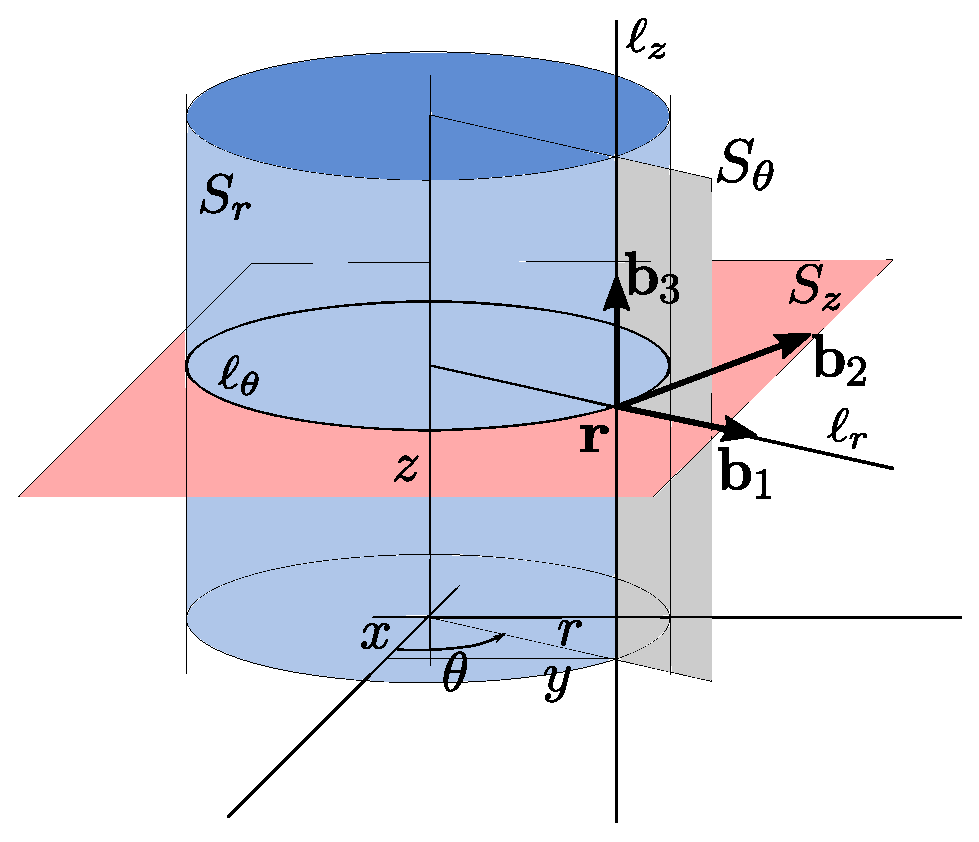
\includegraphics[width=0.45\textwidth]{./fig/cylindricalCoordinates.eps}\label{fig:cylCoord:a}}
\quad
\subfloat[][\emph ]
   {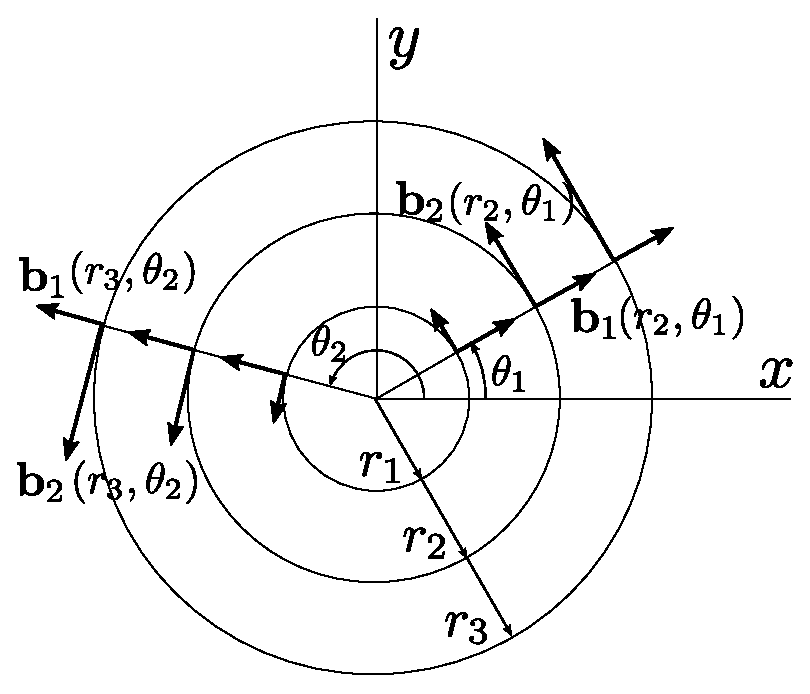
\includegraphics[width=0.45\textwidth]{./fig/cylindricalCoordinatesBasis.eps}\label{fig:cylCoord:b}}
\caption{Sistema di coordinate cilindriche.  \protect\subref{fig:cylCoord:a} Curve e superfici coordinate per un sistema di coordinate cilindriche. \protect\subref{fig:cylCoord:b} Rappresentazione bidimensionale della base naturale - coordinate polari.}\label{fig:cylCoord}
\end{figure}

%Ho appena definito \ref{fig:cylCoord},\ref{fig:cylCoord:a},\ref{fig:cylCoord:b}.

 \subsection{Tensore metrico.}
%
\vspace{15pt}
\begin{definition}[Tensore metrico]
 Il tensore metrico è un tensore del secondo ordine (o meglio un campo tensoriale, poiché in generale è funzione della coordinata spaziale) definito come il tensore le cui componenti covarianti $g_{ik}$ e contravarianti $g^{ik}$ sono rispettivamente i prodotti scalari dei vettori $\bm{b}_i$ della base naturale e dei vettori della base reciproca $\bm{b}^i$. Il tensore metrico $\bm{g}$ viene scritto nella base prodotto naturale e nella sua reciproca come
\begin{equation}
  \bm{g} = g_{ij} \bm{b}^i \otimes \bm{b}^j = g^{ij} \bm{b}_i \otimes \bm{b}_j ,
\end{equation}
con le componenti definite come
 \begin{equation}\label{eqn:defTensoreMetrico}
   g_{ij} = \bm{b}_i \cdot \bm{b}_j , \qquad g^{ij} = \bm{b}^i \cdot \bm{b}^j .
 \end{equation}
\end{definition}
%
% Si definisce il \textbf{tensore metrico} $\bm{g} = g_{ij} \bm{b}^i \otimes \bm{b}^j
% = g^{ij} \bm{b}_i \otimes \bm{b}_j $
% \begin{equation}
%   g_{ij} = \bm{b}_i \cdot \bm{b}_j \qquad , \qquad g^{ij} = \bm{b}^i \cdot \bm{b}^j
% \end{equation}
\begin{remark}
 Il tensore metrico è simmetrico.
\end{remark}
 Il tensore metrico caratterizza la geometria dello spazio (o meglio della varietà $\bm{x}(q^i)$ descritta dai parametri $q^i$). I concetti quali distanza, angolo, lunghezza di una curva possono essere espressi in funzione del tensore metrico $\bm{g}$. Ad esempio, è possibile scrivere la lunghezza $ds$ dell'elemento elementare $d\bm{x} = \dfrac{\partial \bm{x}}{\partial q^i} dq^i = \bm{b}_i dq^i$ come
 \begin{equation}
  ds^2 = |d\bm{x}|^2 = d\bm{x} \cdot d\bm{x} = \left( \bm{b}_i dq^i \right) \cdot \left(  \bm{b}_j dq^j\right) = \bm{b}_i \cdot \bm{b}_j dq^i dq^j = g_{ij} dq^i dq^j ,
 \end{equation}
 dove, come sempre, sono sottointese le sommatorie sugli indici ripetuti.
%
\noindent
Come già visto in precedenza, il tensore metrico risulta utile nel passaggio dalla componenti contravarianti a quelle 
 covarianti e viceversa, consentendo di esprimere un vettore della base $\{ \bm{b}_k \}$ nella base $\{ \bm{b}^k \}$ e viceversa tramite le (\ref{eqn:xxx})
 \begin{equation}
\bm{b}_i = g_{ik} \bm{b}^k , \quad \bm{b}^i = g^{ik} \bm{b}_k ,
 \end{equation}
 con $g_{ij} = \bm{b}_i \cdot \bm{b}_j$ e $g^{ij} = \bm{b}^i \cdot \bm{b}^j$. In maniera analoga è possibile passare dalle coordinate contravarianti a quelle covarianti e viceversa tramite le (\ref{eqn:xxx}). Ad esempio, per un vettore $\bm{v} = v^i \bm{b}_i = v_i \bm{b}^i$, 
 \begin{equation}
  v^i = g^{ik} v_k , \qquad v_i = g_{ik} v^k .
 \end{equation}
 Sempre secondo le (\ref{eqn:xxx}), per un tensore del secondo ordine $\bm{S}= S^{ij} \bm{b}_i \otimes \bm{b}_j = 
    S^{i\ }_{\ j} \bm{b}_i \otimes \bm{b}^j =
    S^{\ j}_{i\ } \bm{b}^i \otimes \bm{b}_j = 
    S_{ij} \bm{b}^i \otimes \bm{b}^j$ si ottiene
 \begin{equation}
  S^{ij} = g^{jk} S^{i\ }_{\ k} = g^{ik} S^{\ \ j}_{k\ } = g^{ik} g^{jl} S_{kl} .
 \end{equation}
%
\begin{example}[Coordinate cartesiane]
    Poichè i vettori della base naturale sono costanti e ortonormali in tutto lo spazio, dalla definizione (\ref{eqn:defTensoreMetrico}) segue che il tensore metrico $g_{ik}$ è uguale all'identità.
 La lunghezza dell'elemento di linea infinitesimo è uguale a
\begin{equation}
    ds^2 = |d\bm{x}|^2 = dx^2 + dy^2 + dz^2 \ .
\end{equation}
\end{example}
%
\begin{example}[Coordinate cilindriche]
 Svolgendo i prodotti scalari tra i vettori della base del sistema di coordinate cilindriche, le componenti $g_{ik}$ del tensore metrico possono essere raccolte nella matrice.
\begin{equation}
 \begin{bmatrix} g_{rr} & g_{r\theta} & g_{rz} \\
 g_{\theta r} & g_{\theta \theta} & g_{\theta z} \\
 g_{z r} & g_{z \theta} & g_{zz} \\ \end{bmatrix} = 
 \begin{bmatrix} 1 & 0 & 0 \\ 0 & r^2 & 0 \\ 0 & 0 & 1  \\ \end{bmatrix} .
\end{equation}
 Il tensore metrico è diagonale, poichè la base è ortogonale. Le componenti covarianti $g^{ik}$ del tensore metrico si ottengono dall'inversione dei simboli $g_{ik}$
\begin{equation}
 \begin{bmatrix} g^{rr} & g^{r\theta} & g^{rz} \\
 g^{\theta r} & g^{\theta \theta} & g^{\theta z} \\
 g^{z r} & g^{z \theta} & g^{zz} \\ \end{bmatrix} = 
 \begin{bmatrix} 1 & 0 & 0 \\ 0 & r^{-2} & 0 \\ 0 & 0 & 1  \\ \end{bmatrix} .
\end{equation}
La base reciproca è $\bm{b}^r = \bm{b}_r$, $\bm{b}^{\theta} = r^{-2} \bm{b}_{\theta} = r^{-1} \bm{\hat{\theta}}$, $\bm{b}^z = \bm{b}_z$.
 La lunghezza dell'elemento di linea infinitesimo è uguale a
\begin{equation}
    ds^2 = |d\bm{x}|^2 = dr^2 + r^2 d\theta^2 + dz^2 \ .
\end{equation}
\end{example}


% \paragraph{Componenti contravarianti, covarianti e fisiche.} \dots
 
 \subsection{Simboli di Christoffel.} 
I vettori della base naturale $\bm{b}_i$ sono definiti come le derivate parziali del vettore posizione $\bm{x}$ rispetto alle coordinate $q^i$ utilizzate per descrivere lo spazio. In generale, quindi anche i vettori della base naturale non sono costanti nello spazio, ma sono funzioni delle coordinate $q^i$. Se i vettori della base variano dello spazio, le loro derivate rispetto ai parametri $q^i$ non sono nulle e possono essere espresse nella base naturale e nella base reciproca come
\begin{equation}\label{eqn:dbdq}
 \dfrac{\partial \bm{b}_i}{\partial q^j} = \Gamma_{ij}^k \bm{b}_k ,
\end{equation}
 dove stati introdotti i simboli di Christoffel di secondo tipo $\Gamma^{k}_{ij}$. In particolare, dalla (\ref{eqn:dbdq}), i simboli di Christoffel di secondo tipo $\Gamma^{k}_{ij}$ possono essere definiti come la $k$-esima componente contravariante della derivata $\partial \bm{b}_i/\partial q^j$. Sfruttando la definizione di base reciproca, è possibile calcolare i simboli di Christoffel dalle (\ref{eqn:dbdq}) come
\begin{equation}
  \Gamma^{k}_{ij} = \dfrac{\partial \bm{b}_i}{\partial q^j} \cdot \bm{b}^k .
\end{equation}
Essendo le componenti delle derivate prime dei vettori della base naturale, a sua volta derivate prime del vettore posizione, i simboli di Christoffel rappresentano le componenti delle derivate seconde del vettore posizione $\bm{x}$ rispetto alle coordinate $q^i$,
\begin{equation}
 \Gamma_{ji}^k \bm{b}_k = 
 \dfrac{\partial \bm{b}_j}{\partial q^i} =\dfrac{\partial^2 \bm{x}}{\partial q^j \partial q^i} =
 \dfrac{\partial^2 \bm{x}}{\partial q^i \partial q^j} = \dfrac{\partial \bm{b}_i}{\partial q^j}= \Gamma_{ij}^k \bm{b}_k ,
\end{equation}
dove l'uguaglianza delle derivate seconde miste è verificata sotto le ipotesi del \textit{teorema di Schwarz}. Uguagliando le componenti alle estremità dell'uguaglianza precedente, si ottengono le condizioni di simmetria per i simboli di Christoffel,
\begin{equation}
 \Gamma_{ji}^k = \Gamma_{ij}^k \ .
\end{equation}
\begin{remark}
 I simboli di Christoffel \textbf{non} costituiscono le componenti di un tensore, poichè non seguono la (\ref{eqn:t2t:t}) nel cambio di sistemi di coordinate.
\end{remark}

\begin{example}[Coordinate cartesiane]
 Poichè i vettori della base naturale sono costanti in tutto lo spazio, i simboli di Christoffel per il sistema di coordinate cartesiane sono identicamente nulli.
\end{example}
\begin{example}[Coordinate cilindriche]
 Vengono calcolati i simboli di Christoffel di secondo tipo, che verranno poi utilizzati in seguito). Da un calcolo diretto dei simboli di Christoffel di secondo tipo, si ottiene che gli unici simboli di Christoffel diversi da zero sono
\begin{equation}
 \Gamma^2_{21} = \Gamma^2_{12} = r^{-1} , \quad \Gamma^1_{22} = - r ,
\end{equation}
dove l'indice 1 è associato alla coordinata $r$, l'indice 2 alla coordinata $\theta$. Infatti
\begin{equation}
\begin{aligned}
 \Gamma_{21}^2 = \Gamma_{12}^2  & = \dfrac{\partial \bm{b}_1}{\partial q^2} \cdot \bm{b}^2 = \dfrac{\partial \bm{\hat{r}}}{\partial \theta} \cdot( r^{-1} \bm{\hat{\theta}} ) = \bm{\hat{\theta}} \cdot (r^{-1} \bm{\hat{\theta}}) = r^{-1} \\
 \Gamma_{22}^1  & = \dfrac{\partial \bm{b}_2}{\partial q^2} \cdot \bm{b}^1 = \dfrac{\partial (r \bm{\hat{\theta}})}{\partial \theta} \cdot \bm{\hat{r}} = - r \bm{\hat{r}} \cdot \bm{\hat{r}} = - r . \\
\end{aligned}
\end{equation}
\end{example}

% +++++++++++++++++++++++++++++++++++++++++++++++++++++++++++++++++++++++++++++++++
\section{Operatori differenziali}\label{ch:operatoriDiff}
 % \paragraph{Derivata covariante}
 % \paragraph{Operatori differenziali}
 % \paragraph{Gradiente}
 % \paragraph{Divergenza}
 % \paragraph{Laplaciano}
 % \paragraph{Rotore}
 % \paragraph{Operatore di advezione}
In questo paragrafo vengono definiti alcuni operatori differenziali sui campi tensoriali, cioè tensori che sono funzioni dello spazio. Un operatore è una funzione che prende come argomento l'oggetto al quale viene applicato, per restituirne un altro. In termini generali, un operatore $P: U \rightarrow V$, prende un elemento di $U$ e ne restituisce uno di $V$,
\begin{equation}\label{def:operatore}
  \bm{v} = P(\bm{u}),
\end{equation}
con $\bm{u} \in U$, $\bm{v} \in V$. Per ottenere un vettore di $\bm{v} \in V$, l'operatore $P$ deve avere come argomento (deve essere applicato a) un elemento $\bm{u} \in U$. Se $P$ è un operatore lineare spesso si possono omettere le parentesi e indicare semplicemente $\bm{v}=P\bm{u}$.
L'ordine di un operatore coincide con il massimo ordine delle derivate (in questo caso spaziali) contenute nella definizione dell'operatore. Inizialmente vengono introdotti gli operatori di primo ordine che non richiedono l'introduzione di prodotti esterni (parenti dei prodotti vettoriali): gradiente, divergenza e operatore di advezione. Viene poi introdotto l'operatore di rotore di un campo vettoriale, limitandosi a sistemi di coordinate cartesiane. Infine viene introdotto il laplaciano, un operatore del secondo ordine definito come la divergenza del gradiente.
\begin{remark}
 Diversi autori usano convenzioni diverse per la definizione degli operatori differenziali, come ad esempio la divergenza di un tensore di secondo ordine. Nel caso di tensori simmetrici (come sono i tensori degli sforzi per materiali non polari), le due diverse definizioni di divergenza di un tensore portano allo stesso risultato, grazie alla simmetria del tensore. 
\end{remark}

\subsection{Gradiente}
L'operatore di gradiente è connesso alla derivata direzionale di un campo tensoriale.
L'operatore di gradiente alza di 1 l'ordine del tensore al quale viene applicato.
\begin{operator}[Gradiente] 
    In particolare, nel punto $\bm{x}$ la derivata direzionale di un tensore $\bm{T}$ in una qualsiasi direzione $\bm{c}$ di un campo tensoriale è il prodotto scalare tra il gradiente del tensore e il vettore $\bm{c}$,
 \begin{equation}\label{eqn:grad:def}
   \bm{c} \cdot \bm{\nabla} \bm{T}(\bm{x}) = \left. \dfrac{d}{d\alpha} \bm{T}(\bm{x}+\alpha\bm{c})\right|_{\alpha=0} \ .
 \end{equation}
\end{operator}
%
\noindent
Il gradiente del tensore $\bm{T}$ può essere scritto sfruttando la definizione della base naturale e della sua reciproca come
%\begin{fBox}
 \begin{equation}\label{eqn:grad:natural}
  \bm{\nabla} \bm{T} = \bm{b}^i \otimes \dfrac{\partial \bm{T}}{\partial q^i} ,
 \end{equation}
%\end{fBox}
dove i vettori $\bm{b}^i$ sono quelli della base reciproca della base naturale e, come al solito, è sottintesa la sommatoria sugli indici ripetuti.
%  \'E possibile indicare l'operatore gradiente con $G$, senza applicarlo ad alcun tensore, rimuovendo l'argomento dalla (\ref{eqn:grad:natural}),
%  \begin{equation}\label{eqn:grad:natural:operator}
%   G \underline{\hspace{8pt}} = \text{grad} \ \underline{\hspace{8pt}} = \dfrac{\partial \underline{\hspace{8pt}}}{\partial q^i} \otimes \bm{b}^i ,
%  \end{equation}
%  avendo lasciato lo spazio $\underline{\hspace{8pt}}$ per inserire l'argomento dell'operatore gradiente e avendo omesso le parentesi poichè il gradiente è un operatore lineare. Il gradiente di un campo tensoriale $\bm{T}$ viene ottenuto semplicemente inserendo $\bm{T}$ negli spazi indicati nella (\ref{eqn:grad:natural:operator}).
%
 \noindent
 Il gradiente di un tensore di ordine $r$ ha ordine $r+1$. Per esempio, il gradiente di un campo scalare $f$ è il vettore $\bm{\nabla} f$
 \begin{equation}\label{eqn:grad:scalar}
  \bm{\nabla} f = \bm{b}^i \dfrac{\partial f}{\partial q^i} = \dfrac{\partial f}{\partial q^i} \bm{b}^i = \dfrac{\partial f}{\partial q^k} g^{ik} \bm{b}_i \ ,
 \end{equation}
 avendo utilizzato la relazione $\bm{b}^i = g^{ik} \bm{b}_k$ tra i vettori di una base e quelli della sua reciproca (e avendo ``invertito'' gli indici ripetuti, che vengono saturati dalle sommatorie).
 Il gradiente di un campo vettoriale è il campo tensoriale del secondo ordine che viene scritto nella base naturale come
 \begin{equation}\label{eqn:grad:vector}
   \bm{\nabla} \bm{v} = \bm{b}^i \otimes \dfrac{\partial \bm{v}}{\partial q^i} = \left[ \dfrac{\partial v^i}{\partial q^k} + \Gamma_{lk}^i v^l \right] \bm{b}^k \otimes \bm{b}_i ,
 \end{equation}
dove sono sottointese le sommatorie sugli indici ripetuti.
\begin{exercise}[Gradiente di un campo vettoriale] Ricavare l'espressione (\ref{eqn:grad:vector}) del gradiente di un campo scalare.

 \vspace{5pt}\noindent
 \textbf{Soluzione.} \'E possibile ricavare questa espressione tramite calcolo diretto delle derivate parziali di $\bm{v}$, ricordandosi la definizione dei simboli di Christoffel e, alla fine, ricordandosi che è possibile scambiare gli indici che vengono saturati da sommatoria, \vspace{-5pt}
\begin{equation}
\begin{aligned}
    \bm{\nabla} \bm{v} & = \bm{b}^k \otimes \dfrac{\partial \bm{v}}{\partial q^k} % = \\
       = \bm{b}^k \otimes \dfrac{\partial (v^i \bm{b}_i)}{\partial q^k}  = \\
     & = \bm{b}^k \otimes \left[ \dfrac{\partial v^i }{\partial q^k} \bm{b}_i +
       v^i \dfrac{\partial \bm{b}_i}{\partial q^k} \right] % = \\
       = \bm{b}^k \otimes \left[ \dfrac{\partial v^i }{\partial q^k} \bm{b}_i +
       v^i \Gamma^{l}_{ik} \bm{b}_l \right] = \\
     & = \left[ \dfrac{\partial v^i }{\partial q^k} +
       v^l \Gamma^{i}_{lk} \right] \bm{b}^k \otimes \bm{b}_i = \nabla_k v^i \bm{b}^k \otimes \bm{b}_i \ ,
\end{aligned}
\end{equation}
dove è stata introdotta la derivata covariante $\nabla_k v^i$ della componente $v^i$ del vettore, rispetto alla coordinata $q^k$.
\end{exercise}

\noindent
Il gradiente di un campo tensoriale del secondo ordine $\bm{S}$ è il campo tensoriale del terzo ordine
 \begin{equation}\label{eqn:grad:tensor2}
   \bm{\nabla} \bm{S} = \left[ \dfrac{\partial S^{ij}}{\partial q^k} + \Gamma_{kl}^i S^{lj} + \Gamma_{kl}^j S^{il} \right]
                \bm{b}^k \otimes \bm{b}_i \otimes \bm{b}_j =: \nabla_k S^{ij} \bm{b}^k \otimes \bm{b}_i \otimes \bm{b}_j \ ,
 \end{equation}
 dove è stata introdotta la definizione di \textbf{derivata covariante} $\nabla_k S^{ij}$ della componente $S^{ij}$ rispetto alla coordinata $q^k$, come generalizzazione delle derivate parziali. Un campo tensoriale è costante nello spazio se sono nulle tutte le sue derivate covarianti.
\begin{exercise}[Gradiente di un campo tensoriale del secondo ordine]
 Aiutandosi con la dimostrazione data per il gradiente di un campo vettoriale, dimostrare che il gradiente di un campo tensoriale del secondo ordine ha l'espressione (\ref{eqn:grad:tensor2}) utilizzando la base naturale e la sua reciproca.
\end{exercise}
%
\begin{example}[Coordinate cartesiane]
 Poichè la base naturale e la sua reciproca coincidono con la base ortonormale $\{\bm{\hat{x}}, \bm{\hat{y}}, \bm{\hat{z}}\}$ e tutti i simboli di Christoffel per le coordinate cartesiane sono nulli, dalla (\ref{eqn:grad:scalar}) si ottiene la forma già nota del gradiente di un campo scalare $f$
\begin{equation}
 \bm{\nabla} f = \dfrac{\partial f}{\partial x} \bm{\hat{x}} +
                 \dfrac{\partial f}{\partial y} \bm{\hat{y}} +
                 \dfrac{\partial f}{\partial z} \bm{\hat{z}} .
\end{equation}
Il gradiente di un vettore $\bm{v} = v^1 \bm{b}_1 +v^2 \bm{b}_2 + v^3 \bm{b}_3  = v_x \bm{\hat{x}} + v_y \bm{\hat{y}} + v_z \bm{\hat{z}}$ è
\begin{equation}
 \begin{aligned}
  \bm{\nabla} \bm{v} = & \p{v_x}{x} \bh{x}\ot\bh{x} + 
                         \p{v_y}{x} \bh{x}\ot\bh{y} +
                         \p{v_z}{x} \bh{x}\ot\bh{z} + \\ 
                     + & \p{v_x}{y} \bh{y}\ot\bh{x} + 
                         \p{v_y}{y} \bh{y}\ot\bh{y} +
                         \p{v_z}{y} \bh{y}\ot\bh{z} + \\ 
                     + & \p{v_x}{z} \bh{z}\ot\bh{x} + 
                         \p{v_y}{z} \bh{z}\ot\bh{y} +
                         \p{v_z}{z} \bh{z}\ot\bh{z} , \\ 
 \end{aligned}
\end{equation}
 le cui componenti possono essere raccolte nella matrice
\begin{equation}
 \begin{bmatrix}
  \p{v_x}{x}  & 
  \p{v_y}{x}  &
  \p{v_z}{x}   \\ 
  \p{v_x}{y}  & 
  \p{v_y}{y}  &
  \p{v_z}{y}   \\ 
  \p{v_x}{z}  & 
  \p{v_y}{z}  &
  \p{v_z}{z}   \\ 
 \end{bmatrix} \ ,
\end{equation}
avendo associato l'indice di riga al primo vettore della base prodotto e l'indice di colonna al secondo vettore della base prodotto.
\end{example}
%
\begin{example}[Coordinate cilindriche]
 Il gradiente in coordinate cilindriche di un campo scalare $f$ può essere scritto nella base ortonormale $\{ \bh{r}, \bh{\theta},\bh{z} \}$ come
\begin{equation}
 \bm{\nabla} f = \p{f}{r} \bh{r} + \dfrac{1}{r}\p{f}{\theta} \bh{\theta} +
   \p{f}{z} \bh{z} ,
\end{equation}
 avendo utilizzato la (\ref{eqn:grad:scalar}) ed essendosi ricordati che $\bh{b}_2 = \bh{\theta} / r$. Da quest'ultima relazione tra i vettori delle basi naturale e ortonormale si ottiene il legame $v^2 = r v_{\theta}$ tra le componenti del vettore $\bm{v} = v^1 \bh{b}_1 + v^2 \bh{b}_2 + v^3 \bh{b}_3 = v_r \bh{r} + v_{\theta} \bh{\theta} + v_z \bh{z}$ espresse in queste basi. Utilizzando queste relazioni nella formula (\ref{eqn:grad:vector}) del gradiente di un campo vettoriale, è possibile scrivere
\begin{equation}
\begin{aligned}
    \bm{\nabla} \bm{v} & = \left[ \dfrac{\partial v^i}{\partial q^k} + \Gamma_{lk}^i v^l \right] \bm{b}^k \otimes \bm{b}_i = \\
     & = \frac{\partial v^1}{\partial q^1}                                   \bm{b}^1 \otimes \bm{b}_1   + 
        \left( \frac{\partial v^1}{\partial q^2} + \Gamma_{22}^1 v^2 \right) \bm{b}^2 \otimes \bm{b}_1   + 
        \frac{\partial v^1}{\partial q^3}                                    \bm{b}^3 \otimes \bm{b}_1   + \\
     & + \left( \frac{\partial v^2}{\partial q^1} + \Gamma_{21}^2 v^2 \right)\bm{b}^1 \otimes \bm{b}_2   + 
        \left( \frac{\partial v^2}{\partial q^2} + \Gamma_{12}^2 v^1 \right) \bm{b}^2 \otimes \bm{b}_2   + 
        \frac{\partial v^2}{\partial q^3}                                    \bm{b}^3 \otimes \bm{b}_2   + \\
     & + \frac{\partial v^3}{\partial q^1}                                   \bm{b}^1 \otimes \bm{b}_3   + 
        \frac{\partial v^3}{\partial q^2}                                    \bm{b}^2 \otimes \bm{b}_3   + 
        \frac{\partial v^3}{\partial q^3}                                    \bm{b}^3 \otimes \bm{b}_3   = \\
     & = \frac{\partial v_r}{\partial r}                                           \bm{\hat{r}}      \otimes \bm{\hat{r}}       + 
        \frac{1}{r}\left( \frac{\partial v_r}{\partial \theta} - v_\theta \right)  \bm{\hat{\theta}} \otimes \bm{\hat{r}}       + 
        \frac{\partial v_r}{\partial z}                                            \bm{\hat{z}}      \otimes \bm{\hat{r}}       + \\
     & +  \frac{\partial v_\theta}{\partial r}                                     \bm{\hat{r}}      \otimes \bm{\hat{\theta}}  + 
        \frac{1}{r}\left( \frac{\partial v_\theta}{\partial \theta} +  v_r \right) \bm{\hat{\theta}} \otimes \bm{\hat{\theta}}  + 
        \frac{\partial v_\theta}{\partial z}                                       \bm{\hat{z}}      \otimes \bm{\hat{\theta}}  + \\
     & + \frac{\partial v_z}{\partial r}                                           \bm{\hat{r}}      \otimes \bm{\hat{z}}       + 
        \frac{1}{r}\frac{\partial v_z}{\partial \theta}                            \bm{\hat{\theta}} \otimes \bm{\hat{z}}       + 
        \frac{\partial v_z}{\partial z}                                            \bm{\hat{z}}      \otimes \bm{\hat{z}}        ,
\end{aligned}
\end{equation}
 avendo utilizzato i valori dei simboli di Christoffel ricavati in precedenza. Si noti come l'annullarsi delle derivate parziali delle componeti del vettore non implichi l'uniformità (costanza in spazio e quindi gradiente nullo) del campo vettoriale: devono annullarsi le derivate covarianti poichè un campo vettoriale uniforme espresso in coordinate cilindriche (come in ogni altro sistema di coordinate diverso da quello cartesiano) non ha componenti costanti in spazio.
\end{example}

% ===============================================================
\subsection{Divergenza}
L'operatore divergenza è associato all'idea di densità di flusso\footnote{Si può ricavare questa interpretazione dal teorema della divergenza.} e può essere definito come contrazione del gradiente del campo al quale viene applicata. L'operatore di divergenza quindi abbassa di 1 (il gradiente alza di 1 l'ordine, la contrazione di due indici lo abbassa di 2) l'ordine del campo tensoriale al quale è applicata. Non può quindi essere applicata a un campo scalare (tensore di ordine 0).
\begin{operator}[Divergenza]
 La divergenza di un campo tensoriale è definito dalla contrazione degli ultimi due indici del gradiente del campo tensoriale stesso.
\begin{equation}\label{eqn:div:def}
 \bm{\nabla} \cdot \bm{T} = \bm{C}^{1}_{2} \big( \bm{\nabla} \bm{T} \big)\  .
\end{equation}
\end{operator}
% L'operatore di divergenza abbassa di 1 l'ordine del tensore al quale viene applicato: la divergenza di un tesnore di ordine $r$ ha ordine $r-1$. Non può quindi essere applicato a un campo scalare (tensore di ordine 0).
La divergenza di un campo vettoriale espresso nella base naturale è
\begin{equation}\label{eqn:div:vector}
 \bm{\nabla} \cdot\bm{v} = \dfrac{\partial v^{i}}{\partial q^i} + \Gamma_{il}^i v^{l} = \nabla_i v^{i} .
\end{equation}
 La divergenza di un tensore $\bm{S}$ del secondo ordine è il campo vettoriale $\bm{\nabla} \cdot \bm{S}$ che viene scritto nella base naturale come
 \begin{equation}\label{eqn:div:tensor2}
  \bm{\nabla} \cdot \bm{S} = \left[ \dfrac{\partial S^{ij}}{\partial q^i} + \Gamma_{il}^i S^{lj} + \Gamma_{il}^j S^{il} \right] \bm{b}_j .
 \end{equation}
%
Questo operatore può essere espresso tramite la derivata covariante come
\begin{equation}
 \bm{\nabla} \cdot \bm{S} = \nabla_i S^{ij} \bm{b}^j ,
\end{equation}
e può essere pensato come il prodotto ``dot'' tra il ``vettore formale'' $\bm{\nabla} = \nabla_k \bm{b}^k$ e il tensore $S^{ij} \bm{b}_i \otimes \bm{b}_j$,
\begin{equation}
      \bm{\nabla} \cdot \bm{S} = (\nabla_k \bm{b}^k) \cdot ( S^{ij} \bm{b}_i \otimes \bm{b}_j ) = \nabla_k S^{ij} \underbrace{\bm{b}^k \cdot \bm{b}_i}_{\delta^k_i} \otimes \bm{b}_j  = 
     \nabla_i S^{ij} \bm{b}_j \ . 
\end{equation}
%

\begin{exercise}
 Utilizzando la definizione di divergenza e l'espressione (\ref{eqn:grad:vector}) del gradiente di un campo vettoriale, ricavare l'espressione (\ref{eqn:div:vector}) di un campo vettoriale.
\end{exercise}
\begin{exercise}
 Utilizzando la definizione di divergenza e l'espressione (\ref{eqn:grad:tensor2}) del gradiente di un campo vettoriale, ricavare l'espressione (\ref{eqn:div:tensor2}) di un campo vettoriale.
\end{exercise}

% \noindent
% La divergenza di un vettore $\bm{v}$, questa definizione si riduce alla traccia\footnote{La traccia di un tensore è un \textit{invariante}, cioè non varia cambiando la base dello spazio, definito come la somma degli elementi della diagonale}
% del gradiente
% \begin{equation}
%  \text{div} \bm{v} = \bm{\nabla} \cdot \bm{v}  = \text{tr}(\bm{\nabla}\bm{v})
% \end{equation}
\begin{example}[Coordinate cartesiane]
 Poichè i simboli di Christoffel sono identicamente nulli e i vettori della base naturale coincidono con la terna ortonormale $\{ \bh{x}, \bh{y}, \bh{z}\}$ nei sistemi di coordinate cartesiane, dalla (\ref{eqn:div:vector}) si ottiene la forma già nota della divergenza di un campo vettoriale $\bm{v}$ 
\begin{equation}
 \bm{\nabla} \cdot \bm{v} = \p{v_x}{x} + \p{v_y}{y} + \p{v_z}{z}.
\end{equation}
\end{example}
\begin{example}[Coordinate cilindriche]
In coordinate cilindriche gli unici simboli di Christoffel non nulli sono $\Gamma^2_{12} = \Gamma^2_{21} = r^{-1}$, $\Gamma^1_{22} = -r$. Utilizzando la (\ref{eqn:div:vector}), la divergenza di un campo vettoriale $\bm{v} = v^1 \bh{b}_1 + v^2 \bh{b}_2 + v^3 \bh{b}_3 = v_r \bh{r} + v_{\theta} \bh{\theta} + v_z \bh{z}$ viene scritta in coordinate cilindriche come
\begin{equation}
\begin{aligned}
 \text{div} \bm{v} = \bm{\nabla} \cdot \bm{v} & =
  \p{v^1}{q^1} + \p{v^2}{q^2} + \Gamma_{12}^2 v^1 + \p{v^3}{q^3} = \\
  & = \p{v_r}{r} + \p{ (v_{\theta}/r) }{\theta} + \dfrac{v_r}{r} + \p{v_z}{z} = \\	
  & = \dfrac{1}{r}\p{( r v_r)}{r} + \dfrac{1}{r}\p{v_{\theta}}{\theta} + \p{v_z}{z}.
\end{aligned}
\end{equation}
\end{example}

\begin{remark}
Utilizzando il lemma \ref{lemma:stokes:2} e l'espressione del vettore sforzo (\ref{eqn:tensor:stressTensor}) in componenti cartesiane (per le quali la base reciproca coincide con la base ortonormale naturale e le componenti contravarianti e covarianti coincidono con le variabili fisiche, vedere \S\ref{ch:tensori:coordinate_ortogonali}), è possibile trasformare il contributo degli sforzi di superficie $\bm{t_n}$ in un integrale di volume,
\begin{equation}
  \oint_S \bm{t_n} = \oint_S \bh{n} \cdot \bm{T} = \oint_S n_i T_{ij} = \int_V \partial_i T_{ij} = \int_V \bm{\nabla} \cdot \bm{T} ,
\end{equation}
 avendo indicato la superficie chiusa del volume $V$ con $S=\partial V$ e riconosciuto l'espressione in componenti cartesiane (per le quali le derivate covarianti coincidono con le derivate parziali) dell'operatore $\bm{\nabla} \cdot$ applicato al tensore degli sforzi $\bm{T}$. Poiché il tensore degli sforzi per continui non polari è simmetrico, la confusione generata dalle due definizioni diverse di divergenza usate da alcuni autori è solo apparente quando applicata al tensore degli sforzi.
\end{remark}

\noindent
\begin{remark}
    Le equazioni vettoriali (o tensoriali) e le identità vettoriali (o tensoriali) possono essere scritte nel sistema di riferimento più conveniente. Durante il corso di Fluidodinamica si incontreranno alcune \textbf{identità vettoriali} utili all'elaborazione delle equazioni. Per chi volesse provare a dimostrarle, o dimostrarne almeno qualcuna, può usare le coordinate cartesiane, per le quali i simboli di Christoffel sono nulli e le derivate covarianti si riducono alle derivate parziali. \textbf{La validità di un'identità vettoriale non dipende dal sistema di riferimento in cui viene scritta}. Per fornire un primo esempio, si dimostra che
 \begin{equation}
  \bm{\nabla} \cdot (a \bm{v}) = \bm{\nabla} a \cdot \bm{v} + a \bm{\nabla} \cdot \bm{v} ,
 \end{equation}
 dove $a$ e $\bm{v}$ sono rispettivamente un campo scalare e vettoriale definiti nello spazio $\mathbb{R}^2$. Il campo vettoriale viene scritto in coordinate cartesiane come $\bm{v} = v_x \bh{x} + v_y \bh{y}$. Da un calcolo diretto, si ottiene
 \begin{equation}
 \begin{aligned}
   \bm{\nabla} \cdot (a \bm{v}) & = \p{(a v_x)}{x} + \p{(a v_y)}{y} = \\
    & = \p{a}{x} v_x + a \p{v_x}{x} + \p{a}{y} v_y + a \p{v_y}{y} = \\
    & = \p{a}{x} v_x + \p{a}{y} v_y + a \left(\p{v_x}{x} + \p{v_y}{y} \right) = 
    \bm{\nabla} a \cdot \bm{v} + a \bm{\nabla} \cdot \bm{v} .
 \end{aligned}
 \end{equation}
\end{remark}

% -------------------------------------
\subsection{Operatore di advezione}
L'operatore di advezione comparirà nelle equazioni per rappresentare il trasporto del tensore $\bm{T}$ al quale viene applicato, da parte di un ``campo di velocità'' $\bm{u}$. L'operatore advezione lascia inalterato l'oridne del tensore al quale è applicato.
\begin{operator}[Operatore di advezione] L'operatore di advezione $(\bm{u} \cdot \bm{\nabla})\underline{\hspace{8pt}}$, da parte del campo vettoriale $\bm{u}$, applicato a una quantità tensoriale $\bm{T}$ può essere definito come il prodotto scalare del campo vettoriale $\bm{u}$ con il tensore $\bm{\nabla} \bm{T}$,
 \begin{equation}
  (\bm{u} \cdot \bm{\nabla}) \bm{T} = \bm{u} \cdot \bm{\nabla}\bm{T} .
 \end{equation}
 \end{operator}
 \begin{remark}
  L'operatore di advezione è diverso dall'operatore $\bm{\nabla} \cdot$ applicato al vettore $\bm{u}$. Il prodotto scalare formale tra un vettore, $\bm{u}$, e un vettore formale, $\bm{\nabla}$, non è commutativo. L'operatore $\bm{\nabla} \cdot \underline{\hspace{8pt}}$ è la divergenza e, quando viene applicato a un campo vettoriale $\bm{u}$ restituisce un campo scalare, $d = \bm{\nabla} \cdot \bm{u}$. L'operatore $(\bm{u} \cdot \bm{\nabla})\underline{\hspace{8pt}} $, deve essere applicato a un campo vettoriale $\bm{v}$ per restituire un vettore e non rimanere soltanto un operatore. % Si rimanda all'esempio in coordinate cartesiane
 \end{remark}
 L'operatore di advezione applicato a un campo scalare $f$ viene espresso nella base naturale come
 \begin{equation}
  (\bm{u} \cdot \bm{\nabla})f = \left( u^i \underbrace{\bm{b}_i \cdot \bm{b}^k}_{\delta_i^k} \nabla_k{\underline{\hspace{8pt}}} \right) f  = \left( u^i \nabla_i{\underline{\hspace{8pt}}} \right) f = u^i \nabla_i {f} .
 \end{equation}
 L'operatore di advezione applicato a un campo vettoriale $\bm{v}$ viene espresso nella base naturale come
 \begin{equation}
  (\bm{u} \cdot \bm{\nabla}) \bm{v} = \left( u^i \bm{b}_i \right) \cdot \left( \nabla_{j} v^k \bm{b}^j \ot \bm{b}_k \right) = 
  u^i  \nabla_{j} v^k  \underbrace{\bm{b}_i \cdot \bm{b}^j}_{\delta_i^j} \ot \bm{b}_k = u^i \left[ \p{v^k}{q^j} + \Gamma^k_{jl} v^l \right] \bm{b}_k .
 \end{equation}
 L'operatore di advezione applicato a un campo tensoriale del secondo ordine $\bm{S}$ viene espresso nella base naturale come
 \begin{equation}
  \bm{u} \cdot \bm{\nabla}\bm{S}  =  u^k \nabla_k S^{ij}   \bm{b}_i \otimes \bm{b}_j
    =  u^k \left[  \dfrac{\partial S^{ij}}{\partial q^k} + \Gamma_{kl}^i S^{lj} + \Gamma_{kl}^j S^{il} \right] \bm{b}_i \otimes \bm{b}_j 
 \end{equation}
%
\begin{example}[Coordinate cartesiane]
 L'espressione in coordinate cartesiane dell'operatore di advezione applicato al campo scalare $f$ è
 \begin{equation}
  (\bm{u} \cdot \bm{\nabla}) f = u_x \p{f}{x} + u_y \p{f}{y} + u_z \p{f}{z} = \bm{u} \cdot \bm{\nabla}f .
 \end{equation}
  L'espressione in coordinate cartesiane dell'operatore di advezione applicato al campo vettoriale $\bm{v}$ è
 \begin{equation}
  (\bm{u} \cdot \bm{\nabla}) \bm{v} = (\bm{u} \cdot \bm{\nabla} v_x) \bh{x} + (\bm{u} \cdot \bm{\nabla}v_y) \bh{y} + (\bm{u} \cdot \bm{\nabla}v_z) \bh{z} ,
 \end{equation}
 avendo utilizzato il risultato dell'operatore di advezione applicato a un campo scalare, appena ricavata.
\end{example}
\begin{example}[Coordinate cilindriche]
 L'espressione in coordinate cilindriche dell'operatore di advezione applicato a un campo vettoriale viene fornita in \S\ref{ch:coordCyl}.
\end{example}

\subsection{Rotore}
 Mentre è stato possibile introdurre gli operatore gradiente e divergenza utilizzando gli strumenti del calcolo tensoriale, sarebbe necessario introdurre dei concetti di \textit{Algebra Esterna} per introdurre l'operazione di \textit{prodotto esterno} della quale il rotore di un campo vettoriale è un caso particolare. Essendo questa una prima introduzione al calcolo tensoriale, la trattazione generale di questa operazione (e di molto altro, come ad esempio delle forme differenziali) va ben oltre lo scopo di questo documento.
 Per quanto ci serve, è sufficiente saper operare con il rotore su campi vettoriali e saper esprimere le componenti fisiche del rotore in sistemi di coordinate cartesiane (per le quali la base naturale e la sua base reciproca coincidono con la base ortonormale $\{\bh{x},\bh{y},\bh{z}\}$ e le componenti contravarianti e covarianti coincidono con quelle fisiche).

 \begin{operator}[Rotore]
  Il rotore di un campo vettoriale $\bm{v}$ può essere scritto in coordinate cartesiane tramite l'utilizzo dei simboli $\epsilon_{ijk}$ come
  \begin{equation}
   \text{rot}\bm{v} = \bm{a} = \bm{\nabla} \times \bm{v} , \quad a_i = \epsilon_{ijk} \partial_j v_k ,
  \end{equation}
  dove la derivata parziale $\partial/\partial x_j$ rispetto alla coordinata $x_j$ è stat indicata con $\partial_j$ per brevità.
  I simboli $\epsilon_{ijk}$ assumono valore $1$ se gli indici $\{ijk\}$ formano una permutazione pari di $\{1,2,3\}$,
  $-1$ se gli indici $\{ijk\}$ formano una permutazione dispari di $\{1,2,3\}$, $0$ se ci sono degli indici ripetuti.
  \end{operator}
  Identificando con $1$ la coordinata $x$, con $2$ la coordinata $y$, con $3$ la coordinata $z$, i simboli $\epsilon_{ijk}$ diversi da zero sono
  \begin{equation}
  \begin{aligned}
    \epsilon_{123} = 1 & , \qquad \epsilon_{132} = -1 \\
    \epsilon_{231} = 1 & , \qquad \epsilon_{213} = -1 \\
    \epsilon_{321} = 1 & , \qquad \epsilon_{312} = -1 . \\ 
  \end{aligned}
  \end{equation}
  Le componenti cartesiane del rotore $\bm{a} = \bm{\nabla} \times \bm{v}$ sono
  \begin{equation}
  \begin{cases}
   a_x = \epsilon_{xyz} \partial_y v_z + \epsilon_{xzy} \partial_z v_y = \partial_y v_z - \partial_z v_y  \\
   a_y = \epsilon_{yzx} \partial_z v_x + \epsilon_{yxz} \partial_x v_z = \partial_z v_x - \partial_x v_z  \\
   a_z = \epsilon_{zxy} \partial_x v_y + \epsilon_{zyx} \partial_y v_x = \partial_x v_y - \partial_y v_x .\\
  \end{cases}
  \end{equation}
  Si osservi che si è ottenuto lo stesso risultato che si ottiene usando il determinante simbolico
  \begin{equation}
    \bm{a} = \bm{\nabla} \times \bm{v} = 
    \begin{vmatrix}
     \bm{\hat{x}} & \bm{\hat{y}} & \bm{\hat{z}} \\
     \partial_x   & \partial_y   & \partial_z   \\
     v_x          & v_y          & v_z
    \end{vmatrix} .
  \end{equation}
  %
  \begin{remark}
   I simboli $\epsilon_{ijk}$ possono essere usati anche per esprimere il prodotto vettoriale tra due vettori, caso particolare del prodotto esterno tra tensori. Le componenti cartesiane del prodotto vettoriale $\bm{a} = \bm{b} \times \bm{c}$ sono $a_i = \epsilon_{ijk} b_j c_k$.
  \end{remark}
  %
  \begin{remark}
   I simboli $\epsilon_{ijk}$ rappresentano le componenti dello pseudo-tensore di Levi-Civita, o di Ricci. Solo per curiosità, uno pseudo-tensore si trasforma come un tensore per cambi di coordinate che preservano l'orientazione dello spazio, mentre deve essere aggiunto un segno meno alle componenti se la trasformazione di coordinate cambia l'orientazione dello spazio. Un esempio di trasformazione di coordinate che non conserva l'orientamento dello spazio è una riflessione rispetto a un piano. Ad esempio, date le coordinate cartesiane $(x,y,z)$, la riflessione rispetto al piano $x=0$ è definisce le nuove coordinate come $(q^1,q^2,q^3) = (-x,y,z)$. Se la base $\{\bh{x},\bh{y},\bh{z}\}$ è destrorsa (regola della mano destra), la base naturale nelle coordinate $(q^1,q^2,q^3)$ è sinistrorsa: poichè l'orientazione dello spazio è invertita, bisogna prestare attenzione a svolgere un prodotto vettoriale in questo sistema di coordinate.
  \end{remark}
 
\subsection{Laplaciano}
L'operatore laplaciano è un operatore del secondo ordine, poiché contiene le derivate seconde come derivate di oridne massimo. Questo operatore compare nell'equazione della conduzione del calore e nelle equazioni di Navier--Stokes per rappresentare fenomeni diffusivi\footnote{Poiché queste PDE hanno come la derivata prima nel tempo come derivata temporale di ordine massimo. Non è così nell'equazione delle onde, ma non si può parlare di tutto qui\dots}
 Il laplaciano lascia inalterato l'ordine del tensore al quale è applicato. 
 \begin{operator}[Laplaciano] L'operatore laplaciano è un'operatore del secondo ordine definito come la divergenza del gradiente,
 \begin{equation}
  \Delta \bm{T} = \bm{\nabla} \cdot (\bm{\nabla} \bm{T}) \ .
 \end{equation}
 \end{operator}
 % 
 \begin{example}[Coordinate cartesiane]
  Il laplaciano di un campo scalare $f$ può essere espresso in un sistema di coordinate cartesiane come
  \begin{equation}
   \Delta f = \pp{f}{x} + \pp{f}{y} + \pp{f}{z}.
  \end{equation}
 \end{example}
 \begin{example}[Coordinate cilindriche]
  L'espressione in coordinate cilindriche del laplaciano applicato a campi scalari e vettoriali viene fornita in \S\ref{ch:coordCyl}.
 \end{example} 
 

